\documentclass[tikz,border=8pt]{standalone}
\usepackage{amsmath,amssymb}
\usetikzlibrary{arrows.meta,calc,decorations.markings}

\begin{document}
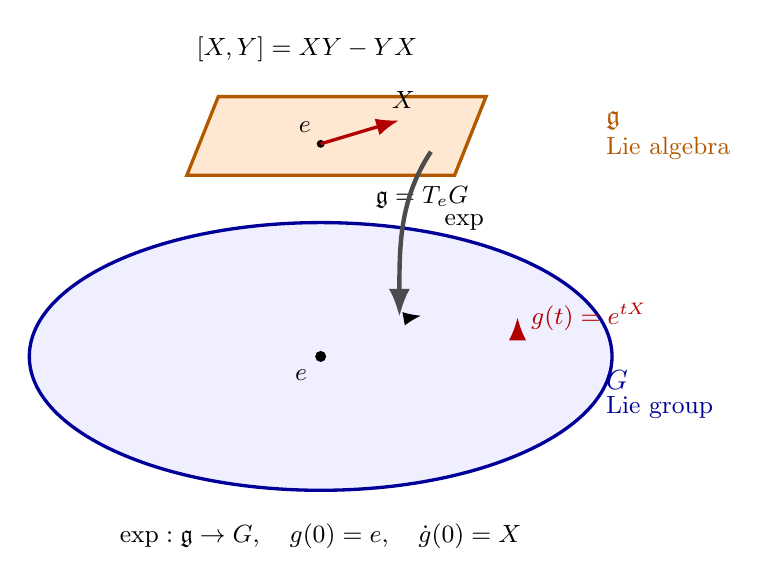
\begin{tikzpicture}[>=Latex]

  % Curved manifold (sphere/ellipse) for G
  \draw[very thick, blue!60!black, fill=blue!10, fill opacity=0.6] (0, 0) ellipse (3.7 and 1.7);

  % point e on manifold
  \fill[black] (0, 0) circle (0.07);
  \node[font=\small, anchor=north east] at (-0.05, -0.05) {$e$};

  % Curve g(t) = e^{tX}
  \draw[->, very thick, red!70!black, decorate, decoration={markings, mark=at position 0.55 with {\arrow{>}}}]
    (0, 0) .. controls (0.8, 0.5) and (1.7, 0.7) .. (2.5, 0.5);
  \node[font=\small, red!70!black, anchor=west] at (2.55, 0.5) {$g(t)=e^{tX}$};

  % Tangent space (slanted) at e
  \begin{scope}[xshift=0cm, yshift=2.7cm]
    \fill[orange!18] (-1.7, -0.4) -- (1.7, -0.4) -- (2.1, 0.6) -- (-1.3, 0.6) -- cycle;
    \draw[very thick, orange!70!black] (-1.7, -0.4) -- (1.7, -0.4) -- (2.1, 0.6) -- (-1.3, 0.6) -- cycle;
    \node[font=\small, anchor=north east] at (2.0, -0.42) {$\mathfrak g = T_e G$};

    % vector X starting at e position projected up
    \fill[black] (0, 0) circle (0.05);
    \node[font=\small, anchor=south east] at (0, 0.02) {$e$};
    \draw[->, very thick, red!70!black] (0, 0) -- (1.0, 0.3);
    \node[font=\small, anchor=south] at (1.05, 0.32) {$X$};

    \node[font=\small, anchor=west] at (-1.7, 1.2) {$[X,Y]=XY-YX$};
  \end{scope}

  % exp arrow
  \draw[->, ultra thick, gray!60!black] (1.4, 2.6) .. controls (1.0, 2.0) and (1.0, 1.4) .. (1.0, 0.5);
  \node[font=\small, anchor=west] at (1.45, 1.7) {$\exp$};

  % G label
  \node[font=\bfseries, blue!60!black, anchor=west] at (3.5, -0.3) {$G$};
  \node[font=\small, blue!60!black, anchor=west] at (3.5, -0.65) {Lie group};
  \node[font=\bfseries, orange!70!black, anchor=west] at (3.5, 3.0) {$\mathfrak g$};
  \node[font=\small, orange!70!black, anchor=west] at (3.5, 2.65) {Lie algebra};

  % bottom formula
  \node[font=\small, anchor=north] at (0, -2.0) {$\exp:\mathfrak g\to G,\quad g(0)=e,\quad \dot g(0)=X$};
\end{tikzpicture}
\end{document}
